Given the difficulty of the problem(s) in the conventional online model, we now consider the case where acceptances are revocable, but rejections are final, a relaxation of the model that is commonly studied for the problem of interval selection. A new interval can now always be accepted by displacing any intervals in the solution conflicting with it. For unit weights, Borodin and Karavasilis \cite{borodin2023any} give an optimal algorithm that is $2k$-competitive, where $k$ is the number of distinct interval lengths. We will refer to this algorithm of \cite{borodin2023any} as the \textit{BK2K} algorithm. \textit{BK2K} is a greedy algorithm, always accepting a new interval when there is no conflict, and whenever a conflict exists, the new interval is accepted only if it is properly included in an interval currently in the solution. We use that as the base logic for our predictions algorithm, and add one more replacement rule, which accepts a new interval $I$ that is only involved in partial conflicts, if $Prd(I) = 1$. Furthermore, an interval accepted by that rule gets marked, to make sure it cannot be replaced by that rule again. We call this algorithm \texttt{Revoke-Unit} \ref{alg:unw-revoke}. Interestingly, this rule of locally \textit{following the predictions once}, suffices to give us $1$-consistency.




\begin{algorithm}
\caption{\texttt{Revoke-Unit}}\label{alg:unw-revoke}
\begin{algorithmic}
\State $M \gets \emptyset$ \Comment{Set of marked intervals}
\State $S \gets \emptyset$ \Comment{Solution set}
\State On the arrival of $I$:
\State $I_{s} \gets $ Set of intervals currently in the solution conflicting with $I$
\If{$I_{s} = \emptyset$ or ($I_{s}=\{I'\}$ and $I \subset I'$)}
    \If{ $I' \in M$}
        \State $M \gets M \cup \{I\}$
    \EndIf
    \State $S \gets S \cup \{I\} \setminus \{I'\} $\Comment{Take $I$ and discard $I'$ if necessary}
\ElsIf{$I$ is only involved in partial conflicts \textbf{and} $Prd(I) = 1$ \textbf{and} $I_{s} \cap M = \emptyset$}
    \State $S \gets S \cup \{I\} \setminus I_s $\Comment{Take $I$ and discard conflicting intervals}
    \State $M \gets M \cup \{I\}$
\EndIf
\end{algorithmic}
\end{algorithm}
%Algorithm \ref{alg:unw-revoke} is a greedy algorithm that uses the same replacement rule (replace when new interval entirely subsumed by existing one) as the optimal $2k$ online algorithm, but has one additional replacement rule for partial conflicts. If the newly arrived interval is only involved in partial conflicts (can only be one or two such conflicts at most), the prediction says it's optimal, and the existing intervals it conflicts with are unmarked (have not been involved in a partial-conflict replacement in the past), then it accepts the new interval. {\color{red} Talk about how follow-the-prediction-ONCE works is the main idea, and suffices for 1-consistency. Also mention the BK2K notation.}

\begin{theorem}
    Algorithm \ref{alg:unw-revoke} achieves $ALG \geq OPT - \eta$.
\end{theorem}
\begin{proof}
    We follow the same approach as in the proof of Theorem \ref{theo:unw-naive-pos}, mapping optimal intervals to intervals taken by the algorithm, and to error. The main difference is that because of revoking, this mapping might be redefined throughout the execution of the algorithm. As before, we let $H$ be the set of error elements, and $H_{I} \subseteq H$ be the set of error elements introduced by $\eta(I)$. Let $I_{opt}$ be an optimal interval. We will define an injective mapping $F: OPT \rightarrow ALG \cup H$ as follows: If $I_{opt}$ is taken by the algorithm, it is initially mapped onto itself. If $I_{opt}$ is later replaced, it must be because of a partial conflict (w.l.o.g. no interval is subsumed by an optimal interval) with a new interval $I'$ with $Prd(I') = 1$. In this case, $I_{opt}$ will be mapped to an error element in $H_{I'}$, or if no further optimal intervals that conflict with $I$ are yet to arrive, it will be mapped to $I$. In both, subcases it will never be remapped.\\
    Consider now the case of $I_{opt}$ being rejected upon arrival. This can only happen if it is involved in (at most two) partial conflicts. There are two possible cases. The first case is that $Prd(I_{opt}) = 0$, and therefore $|H_{I_{opt}}| = 1$, in which case we map $I_{opt}$ to the error element of its own prediction. The second case is that $Prd(I_{opt}) = 1$, but at least one of the conflicting intervals was marked. Let $I_{c}$ be one of the marked, partially conflicting intervals. If $I_{c}$ was marked by being taken through a partial-conflict replacement, it means that $Prd(I_{c}) = 1$, and $|H_{I_{c}} \cup \{I_c\}| > 0$, in which case we can map $I_{opt}$ to an element $h_{c} \in H_{I_{c}}\cup \{I_c\}$.\\
    If $I_{c}$ was instead marked by a proper-inclusion-replacement, we trace the original interval that got marked through a partial-conflict-replacement. Call that interval $I^{'}_{c}$. It holds that $I^{'}_{c}$ conflicts with $I_{c}$, and therefore also conflicts with $I_{opt}$. Moreover, for $I^{'}_{c}$ to have been accepted, it must be that $Prd(I^{'}_{c})=1$ and $|H_{I^{'}_{c}} \cup \{I^{'}_{c}\}|>0$. In this case, we map $I_{opt}$ to an element $h_{c'} \in H_{I^{'}_{c}} \cup \{I^{'}_{c}\}$. In conclusion, we have that $ALG + |H| \geq OPT$, and we get the desired bound.
\end{proof}

We note that the performance of algorithm \ref{alg:unw-revoke} on the instance of Theorem \ref{theo:unw-naive-neg} is exactly equal to $OPT - \eta$, and we get the following lemma.

\begin{lemma}
    The performance of algorithm \ref{alg:unw-revoke} cannot be better than $OPT-\eta$.
\end{lemma}

We next show that the robustness of algorithm \texttt{Revoke-Unit} nearly matches the optimal online guarantee.

\begin{theorem} \label{theo:unw-rev-robust}
    With at most $k$ distinct interval lengths, algorithm \ref{alg:unw-revoke} is $(2k+1)$-robust.
\end{theorem}
\begin{proof}
    We use a charging argument and show that an interval taken by the algorithm can be charged by at most $2k+1$ optimal intervals. As soon as an optimal interval arrives, we map it to an interval already taken by the algorithm or itself. When an interval is replaced during the execution, all optimal intervals charged to it up to that point, will now be charged to the new interval that was accepted. We build upon the proof of Theorem 3.2 in \cite{borodin2023any}. In the case of the \textit{BK2K} algorithm (\cite{borodin2023any}), it is true that for every predecessor trace $\mathcal{P}$, and consecutive intervals $(I_i,I_{i+1}) \in \mathcal{P}$, $\Phi(I_{i+1}) \leq \Phi(I_i) + 2$, and the length of every predecessor trace is at most $k$. While the former is still true for algorithm \texttt{Revoke-Unit}, the latter is not, and that is because we have an additional replacement rule. However, we argue that for every $I_i \in \mathcal{P}$, if $I_j,\; j > i$ is the next interval in the trace that was accepted through proper-inclusion, it is true that $TC(I_j) \leq TC(I_i) + 3$.\\
    
    Figure \ref{fig:pcr-charge} shows how to maximize charge on the event of a partial-conflict replacement. Before being replaced by a partially-conflicting interval, $I_{1}$ can be directly charged by at most two optimal intervals ($I^{1}_{opt}, I^{2}_{opt}$), one on each side. After $I_{2}$ replaces $I_{1}$, it can also be directly charged by two optimal intervals, but only if $I^{2}_{opt}$ was not charged to $I_{1}$ earlier. In other words, if $I_{2}$ is directly charged by two new intervals, it means that $I_{1}$ was directly charged by at most one, concluding that $\Phi(I_2) \leq TC(I_1) + 3$.

    \begin{figure}[H]
	\centering
	
	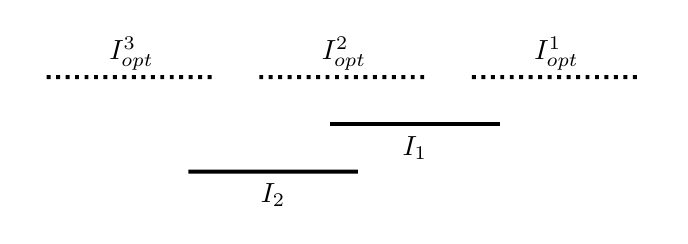
\begin{tikzpicture}[scale=0.6]

	\node at (-5,-1.5) {$I_{2}$};
	\node[draw=none] (I1a) at (-7,-1) {$ $};
	\node[draw=none] (I1b) at (-3,-1) {$ $};
	\draw[line width=0.5mm] (I1a) -- (I1b);
	
	
	%\node[draw=none] (d1) at (-3,-1) {$\rvdots$};

	\node[draw=none] (I2a) at (-5.5,1) {$ $};
	\node[draw=none] (I2b) at (-1.5,1) {$ $};
	\node at (-3.5,1.5) {$I^{2}_{opt}$};
	\draw[dotted,line width=0.5mm] (I2a) -- (I2b);
	
	\node[draw=none] (I3a) at (-10,1) {$ $};
	\node[draw=none] (I3b) at (-6,1) {$ $};
	\node at (-8,1.5) {$I^{3}_{opt}$};
	\draw[dotted,line width=0.5mm] (I3a) -- (I3b);
	
	\node[draw=none] (I4a) at (-4,0) {$ $};
	\node[draw=none] (I4b) at (0,0) {$ $};
	\node at (-2,-0.5) {$I_{1}$};
	\draw[line width=0.5mm] (I4a) -- (I4b);
	
	\node[draw=none] (I5a) at (-1,1) {$ $};
	\node[draw=none] (I5b) at (3,1) {$ $};
	\node at (1,1.5) {$I^{1}_{opt}$};
	\draw[dotted,line width=0.5mm] (I5a) -- (I5b);

	\end{tikzpicture} 
	\caption{Maximum charge through partial-conflict replacement.}\label{fig:pcr-charge}
\end{figure}

Finally, notice that because the mark of an interval carries over when it is replaced, the event of a partial-conflict replacement can occur at most once in each predecessor trace,
and excluding at most one subsequence $(I_i, I_r, I_j) \in \mathcal{P}$ where $TC(I_j) \leq TC(I_i) + 3$, it holds that for $(I_b,I_{b+1}) \in \mathcal{P}$, $\Phi(I_{b+1})\leq \Phi(I_b) + 2$, giving us a worst case competitive ratio of $2k+1$. 
\end{proof}

\begin{corollary}
    With at most $k$ distinct interval lengths, and predictions with total error $\eta$, Algorithm Revoke-Unit achieves $ALG \geq \max\{OPT-\eta , \frac{OPT}{2k+1}\}$.
\end{corollary}

Notice how we can choose not to carry over the mark when proper-inclusion replacement occurs, and get a $3k$-robust algorithm. Such an algorithm is prone to follow the prediction more often, and it can outperform \texttt{Revoke-Unit} for some small values of error caused by adversarial predictions.\\\\
We now look at the case of proportional weights. In the conventional online setting, Garay et al. \cite{garay1997efficient} give a $2\phi + 1  \approx 4.236-$competitive algorithm, while Tomkins \cite{tomkins1995lower} gives a matching lower bound. They call their optimal algorithm \texttt{LR} (for \textit{length of route}), and we include it here for completeness. Unlike the case of unit weights, we now want to accept intervals that occupy as much of the line as possible. Algorithm \texttt{LR} works greedily by always accepting a new interval with no conflicts, and when there are conflicts, it accepts the new interval if its length is at least $\phi$ times greater than the largest conflicting interval. More generally, using parameter $\beta \geq \phi$, we have the following lemma:
\begin{lemma}[Garay et al. \cite{garay1997efficient}]
    Algorithm \texttt{LR} with parameter $\beta \geq \phi$ is $(2\beta + 1)$-competitive for the problem of interval selection with proportional weights.
\end{lemma}
\begin{algorithm}
\caption{LR \cite{garay1997efficient}}\label{alg:garay_prop}
\begin{algorithmic}
\State Parameter $\beta = \phi$ \Comment{optimal value for parameter $\beta$}
\State On the arrival of $I$:
\State $I_{s} \gets $ Set of intervals currently in the solution conflicting with $I$
\If{ $w(I) > \beta \cdot \max\{w(J)\; : \; J\in I_s\}$}
    \State Accept $I$ and displace conflicts
    \State Return
\EndIf
\end{algorithmic}
\end{algorithm}
Instead of using algorithm \texttt{LR} as the base of our predictions algorithm, we consider a slightly modified version, which we refer to as \texttt{LR$'$}, and which compares the weight of the new interval to the sum of the weights of the conflicting intervals, instead of looking only at the longest interval. Although we do not know the exact performance of algorithm \texttt{LR$'$} in the online model, we conjecture it is also $(2\phi + 1)$-competitive.\\\\
In trying to utilize predictions in the case of proportional weights, we first make the following observations:
\begin{observation}
    $1$-consistency is unattainable while maintaining bounded robustness.
\end{observation}
\begin{proof}
    To be $1$-consistent, the algorithm must be able to replace an interval with an arbitrarily smaller one that is part of the optimal solution. The adversary could then stop the instance, forcing arbitrarily bad robustness.
\end{proof}

\begin{observation}
    In order to have bounded robustness, it must be that a new interval that is sufficiently large (small\footnote{More accurately, an interval reducing ALG sufficiently much. }) must always be accepted (rejected).
\end{observation}

\begin{definition}[$\alpha-$increasing]
    An $\alpha$-increasing algorithm never accepts a new conflicting interval
that is less than $\alpha$ times the longest interval it conflicts with.
\end{definition}
\begin{lemma}
    An $\alpha$-increasing algorithm (greedy or non-greedy), cannot be better than $(2\alpha +1)$-consistent.
\end{lemma}
\begin{proof}
    Let an interval $I_1$ arrive first. Let $I_2$ and $I_3$ be intervals that partially conflict with $I_1$ on either side, and $w(I_2) = w(I_3) = \alpha \cdot w(I_1) - \epsilon$. Let $I_4$ with $w(I_4) = w(I_1)-2\epsilon$ be an interval that is fully subsumed by $I_4$. This instance is depicted in figure \ref{fig:neg-alpha-increasing}. The algorithm will never replace $I_1$, while the optimal solution is made of $\{I_2,I_3,I_4\}$.
    \begin{figure}[h] % Adjust the width as needed
        \centering
        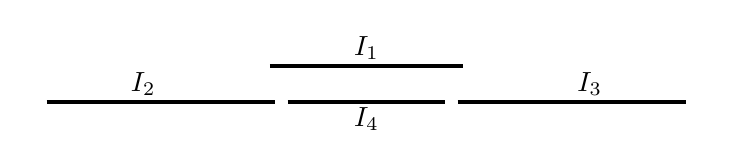
\begin{tikzpicture}[scale=0.45]
	
	\node at (0,0.5) {$I_1$};
	\node[draw=none] (I1a) at (-3,0) {$ $};
	\node[draw=none] (I1b) at (3,0) {$ $};
	\draw[line width=0.5mm] (I1a) -- (I1b);

 \node at (-6.3,-0.5) {$I_2$};
	\node[draw=none] (I2a) at (-9.3,-1) {$ $};
	\node[draw=none] (I2b) at (-2.3,-1) {$ $};
	\draw[line width=0.5mm] (I2a) -- (I2b);

  \node at (6.3,-0.5) {$I_3$};
	\node[draw=none] (I2a) at (2.3,-1) {$ $};
	\node[draw=none] (I2b) at (9.3,-1) {$ $};
	\draw[line width=0.5mm] (I2a) -- (I2b);

	\node[draw=none] (I5a) at (-2.5,-1) {$ $};
	\node[draw=none] (I5b) at (2.5,-1) {$ $};
	\node at (0,-1.5) {$I_{4}$};
	\draw[line width=0.5mm] (I5a) -- (I5b);

	\end{tikzpicture} 
        \caption{Consistency bound for $\alpha$-increasing algorithms.}
        \label{fig:neg-alpha-increasing}
    \end{figure}
\end{proof}
Algorithm \texttt{LR} is a $\phi$-increasing algorithm, while the algorithm by Woeginger \cite{woeginger1994line} for the real-time model is $2$-increasing. Our predictions algorithm \ref{alg:prop-revoke2} \texttt{Revoke-Proportional} is $1$-increasing. The algorithm works like \texttt{LR$'$}, with one additional replacement rule that accepts a new interval that is predicted to be optimal, even if it is not sufficiently larger than what it conflicts with. More precisely, if a new interval is predicted to be optimal and is at least as big as the sum of the weights of the intervals it conflicts with, and none of the conflicting intervals were predicted to be optimal, it will be accepted through the predictions rule. The algorithm takes a parameter $\lambda > 1$, which can be thought of as an indicator of how much the predictions are trusted. As $\lambda$ increases, the consistency bound improves.

\begin{algorithm}
\caption{\texttt{Revoke-Proportional} {\hfil Parameter: $\lambda > 1$ }}\label{alg:prop-revoke2}
\begin{algorithmic}
\State On the arrival of $I$:
\State $I_{s} \gets $ Set of intervals currently in the solution conflicting with $I$
\State Let $w_c = \sum_{J \in I_s} w(J)$ \Comment{Total weight of conflicting intervals}
\If{ $w(I) \geq \lambda\cdot w_c$} \Comment{Main replacement rule}
    \State Accept $I$ and displace conflicts
    \State Return
\ElsIf{$Prd(I) = 1$} \Comment{Predictions rule} 
    \If{($w(I) \geq w_c$ and $|\{J: J \in I_s \text{ and }Prd(J)=1\}| = \emptyset$)} 
    \State Accept $I$ and displace conflicts
    \State Return
    \EndIf
\EndIf
\end{algorithmic}
\end{algorithm}

\begin{theorem}
    Algorithm Revoke-Proportional is $\frac{3\lambda}{\lambda -1}$-consistent.\label{theo:prop-consistent}
\end{theorem}
\begin{proof}
We consider the optimal solution $OPT$ consistent with the fully accurate predictions. We will show that throughout the execution of the algorithm, we have that $\Phi(I) \leq \mu \cdot w(I)$, for every $I$ in the current solution. In the end, we have that $\sum_{I\in ALG} \Phi(I) = OPT$, giving us the $\mu$-consistency of the algorithm.\\\\
As in the proof of Theorem \ref{theo:unw-rev-robust}, we consider the notions of \textit{transfer charge} ($TC$), and \textit{direct charge} ($DC$). We can express $\Phi(I) = TC(I) + DC(I)$. A transfer charge occurs whenever accepting a new interval $I$ replaces intervals currently in the solution. In that case, the total charge of those conflicting intervals is passed on as transfer charge to $I$. Any additional charge to $I$ after its acceptance is through direct charge, namely rejection of subsequent optimal intervals conflicting with $I$. We will write $DC_J(I)$ to denote the amount of direct charge from interval $J$ to interval $I$. Whenever an optimal interval is accepted, we consider its weight being directly charged to itself, and it cannot be directly charged again.\\\\
Whenever an optimal interval is rejected upon arrival, we charge its weight to the intervals it conflicts with, with its weight being distributed to all its conflicting intervals, in proportion to their weight. Specifically, let $I_o$ be the newly arrived optimal interval that is rejected, and $I_s$ denote the set of conflicting intervals. Each interval $J \in I_s$ is directly charged $DC_{I_o}(J)=w(I_o) \frac{w(J)}{w_c}\leq w(I_o)$. Furthermore, for an optimal interval to have been rejected, it must be that even the predictions rule failed, and because the predictions are accurate, it must have failed because $w(I_o) < w_c$. Because of this, we get that $w(I_o) \frac{w(J)}{w_c} \leq w(J)$, and therefore $DC_{I_o}(J)\leq\min\{w(I_o),w(J)\}$. An interval $I \in ALG$ can be directly charged by at most three different types of optimal intervals: 1) smaller intervals that are subsumed by it, 2) an optimal interval partially conflicting on the left, and 3) an optimal interval partially conflicting on the right.
In the case of smaller optimal intervals subsumed by $I$, the total amount of direct charge from those intervals can be at most $w(I)$. Given that each of the two possible partially conflicting intervals can directly charge $I$ at most $w(I)$, we conclude that for every $I\in ALG$:
\begin{equation}
\label{dc-bound}
    DC(I) \leq 3w(I)
\end{equation}
We omitted the case where the rejected optimal interval subsumes $I$, because in that case $DC(I) = w(I)$ and \ref{dc-bound} holds trivially. We now focus on the total amount of charge on any interval $I\in ALG$. Let:
$$\mu = \frac{3\lambda}{\lambda - 1}$$
We want to make sure that throughout the execution of the algorithm, $\Phi(I) \leq \mu \cdot w(I)$. Before any interval is accepted through replacement, intervals in the solution could have only been directly charged through rejected optimal intervals, and because of \eqref{dc-bound}, and the fact that $\lambda > 1$, our desired bound holds. We now consider all the cases of an interval being accepted through replacement.\\\\
\underline{Case $1$}: $I$ is an optimal interval and it is accepted through the predictions rule. In this case we have that $DC(I) = w(I)$, and we need to look at $TC(I)$. Let $L_c$ and $R_c$ denote the intervals (if any) that $I$ is partially conflicting with on the left and on the right respectively, and let $M_c$ denote the set of intervals that $I$ subsumes. We know that all of these conflicting intervals are not optimal, and they were accepted through the algorithm's main rule. First, notice that for all $J\in M_c$, $DC(J) = 0$, and $\Phi(J) = TC(J) \leq \frac{\mu}{\lambda} \cdot w(J)$. Moreover, $L_c$ and $R_c$ had not yet been directly charged by a partially conflicting optimal interval on one side, and therefore we have that $\Phi(L_c) \leq \frac{\mu}{\lambda}\cdot w(L_c) + 2w(L_c)$, and similarly $\Phi(R_c) \leq \frac{\mu}{\lambda}\cdot w(R_c) + 2w(R_c)$.\\
Putting everything together:
\[
\begin{aligned}
    TC(I) &= \sum_{J\in M_c} \Phi(J) + \Phi(L_c) + \Phi(R_c) \\
     & \leq \frac{\mu}{\lambda}\cdot w_c + 2(w(L_c) + w(R_c))\\
     & \leq \left(\frac{\mu}{\lambda} + 2\right)w_c\\
     &\leq \left(\frac{\mu}{\lambda} + 2\right)w(I)
\end{aligned}
\]
The last inequality being true from the fact that the main predictions rule is satisfied. Given also that $DC(I) = w(I)$, we get that $\Phi(I) \leq (\frac{\mu}{\lambda} + 2)w(I) + w(I) = (\frac{\mu}{\lambda} + 3)w(I)$. With our choice of $\mu$, we have:
\[\begin{aligned}
    \Phi(I) &\leq \left(\frac{\frac{3\lambda}{\lambda - 1}}{\lambda} + 3 \right)w(I) \\
    &= \left(\frac{3\lambda}{\lambda -1}\right)w(I)\\\\
\end{aligned}\]
\underline{Case $2$}: $I$ is an optimal interval and it is accepted through the algorithm's main rule. This is similar to case 1, with $DC(I) = w(I)$ and $w(I)\geq \lambda \cdot w_c$. The same analysis gives us $TC(I)\leq \left( \frac{\mu}{\lambda} + 2 \right)\frac{w(I)}{\lambda}$, and because $\lambda > 1$, the same bound holds.\\\\
\underline{Case $3$}: $I$ is not an optimal interval and it is accepted through the algorithm's main rule. In this case we have that $DC(I) \leq 3w(I)$, and we get that
\[\begin{aligned}
    \Phi(I) & \leq \sum_{J\in I_s} \Phi(J) + 3w(I)\\
    & \leq \frac{\mu}{\lambda}\cdot w(I) + 3w(I)\\
    & = \left(\frac{3\lambda}{\lambda -1}\right)w(I)
\end{aligned}\]
In conclusion, we have that throughout the execution of the algorithm, for $I \in ALG$, $\Phi(I)\leq \frac{3\lambda}{\lambda - 1}w(I)$, and therefore $\frac{OPT}{ALG} \leq \frac{3\lambda}{\lambda - 1}$. 
\end{proof}
\vspace{0.5cm}
We see that as $\lambda \rightarrow \infty$, the algorithm's consistency goes to $3$. We now look at the robustness of algorithm \texttt{Revoke-Proportional}.\\
\begin{theorem}
    Algorithm Revoke-Proportional is $\frac{4\lambda^2 + 2\lambda}{\lambda -1}$-robust.
\end{theorem}
\begin{proof}
    The argument is similar to the proof of Theorem \ref{theo:prop-consistent}. Both \textit{direct}, and \textit{transfer} charging work the same way as before. Let $\mu = \frac{2\lambda^2 +3\lambda + 1}{\lambda -1 }$, and $\delta = 2\lambda + 1$. We will show that that for every $I \in ALG$, $\Phi(I)\leq (\mu + \delta)\cdot w(I)=\frac{4\lambda^2 + 2\lambda}{\lambda -1}w(I)$.\\\\
    Notice first that the upper bound on direct charging is not as good as before. More precisely, with $I_o$ being a newly arrived optimal interval that will be rejected and $I_s$ being its conflicting intervals currently in the solution, we have that for every $J\in I_s$, $DC_{I_o}(J)= w(I_o)\frac{w(J)}{w_c}\leq \lambda \cdot w(J)$. More generally, $DC_{I_o}(J) \leq \min\{w(I_o),\lambda\cdot w(J)\}$. As before, given the three different possible types of conflicts, we have that:
    \begin{equation}
        DC(I) \leq (2\lambda + 1)w(I)
    \end{equation}
    We can now bound the total amount of charge on every interval in the algorithm's solution, throughout its execution. Before any replacement happens, the bound $\Phi(I) \leq (\mu + \delta)\cdot w(I)$ holds trivially.\\\\
    \underline{Case $1$}: Interval $I$ is accepted through the algorithm's main rule. We get that:
    \[\begin{aligned}
        \Phi(I) &\leq (\mu + \delta)\cdot w_c + (2\lambda + 1)\cdot w(I)\\
        & \leq (\mu + \delta)\cdot \frac{w(I)}{\lambda} + (2\lambda + 1)\cdot w(I)\\
        & = \left(\frac{\mu + \delta}{\lambda} + 2\lambda + 1\right)w(I)\\
        & = \left( \frac{\frac{4\lambda^2 +2\lambda}{\lambda-1}+2\lambda^2 + \lambda}{\lambda} \right)w(I)\\
        & = \mu \cdot w(I)
    \end{aligned}\]
\underline{Case $2$}: Interval $I$ is accepted through the algorithm's predictions rule. Notice that in this case, all conflicting intervals must have been accepted through the main rule, and not the predictions rule. Because of this, as we showed in case $1$, for every $J\in I_s$, it holds that $\Phi(J) \leq \mu\cdot w(J)$. This helps us bound the amount of transfer charge to interval $I$.
\[\begin{aligned}
    \Phi(I) &\leq \mu \cdot w_c + (2\lambda + 1)\cdot w(I)\\
    & \leq \mu \cdot w(I) + (2\lambda + 1)\cdot w(I) \\
    & = (\mu + \delta)\cdot w(I)
\end{aligned}\]
To summarize, we have shown that in the worst case, $\Phi(I) \leq (\mu + \delta)\cdot w(I)$ for every $I\in ALG$. This concludes the proof.
\end{proof}

\begin{figure*}[t!]
\centering
\caption{\texttt{NASA-iPSC} dataset.} (a) Unit \& Irrevocable, (b) Unit \& Revoking, (c) Proportional \& Irrevocable, (d) Proportional \& Revoking
\includegraphics[width=\textwidth]{exp_pics/nasa/nasa_combined_ann.png}
\label{fig:nasa_exps}
\end{figure*}
\begin{figure*}[t!]
\centering
\caption{\texttt{CTC-SP2} dataset.}
\includegraphics[width=\textwidth]{exp_pics/ctc/ctc_combined_ann.png}
\label{fig:ctc_exps}
\end{figure*}

We note that for $\lambda > \frac{2+\sqrt{5}}{\sqrt{5} -1}\approx 3.42 $, the consistency of our algorithm is already better than $2\phi + 1$, and $22.15$-robust. We have shown we can get consistency better than the online bound of \texttt{LR}, while maintaining bounded robustness. We believe further improvement on the bounds of \texttt{Revoke-Proportional} is possible, with an analysis that looks more closely at the dependence between direct and transfer charging.\\
One may also be able to further improve the algorithm by accepting an interval that is not as big as the sum of its conflicts, making the algorithm $a$-increasing with $a<1$. This would relax the predictions rule further, and make the algorithm more prone to bad choices caused by misleading predictions. In our experiments, we briefly discuss one such algorithm, which we call \texttt{Revoke-Prop-Half}, and which can accept a supposedly optimal interval even if it is half as big as its conflicts.






